\newcommand*{\examnumber}{B135653}
\newcommand*{\field}{Reproducible research and \\resilient supply chains in OpenTTD}
\newcommand*{\tutor}{Bob Fisher}
\newcommand*{\supervisor}{Michael Herrmann}
\newcommand*{\KEYWORDS}{\field, \supervisor, \tutor, School of Informatics, University of Edinburgh}

%
%                       This is a basic LaTeX Template
%                       for the Informatics Research Review

\documentclass[a4paper,11pt]{article}
% Add local fullpage and head macros
\usepackage{head,fullpage}     
% Add graphicx package with pdf flag (must use pdflatex)
\usepackage[pdftex]{graphicx}  
% Better support for URLs
\usepackage{url}
% Date formating
\usepackage{datetime}
% For Gantt chart
\usepackage{pgfgantt}
\usepackage{xcolor}
\usepackage{gnuplottex}
\usepackage[utf8]{inputenc}
\usepackage{fancyvrb}

\definecolor{hyperlinkColor}{HTML}{0D3B68}
\usepackage[shrink=20,stretch=20]{microtype}
\usepackage{siunitx}
\sisetup{detect-all
  ,group-minimum-digits=3% Western convention is groups of 3 digits
  ,mode = text
%   ,text-font-command = \liningroman
}
\usepackage{xurl}
\usepackage{hyperref}
\hypersetup{%
   pdfauthor=\texorpdfstring{\examnumber}{\examnumber}%
  ,pdftitle=\texorpdfstring{\field}{\field}%
  ,pdfsubject=\texorpdfstring{\field}{\field}%
  ,pdfkeywords=\texorpdfstring{\KEYWORDS}{\KEYWORDS}%
  ,linktoc=all%
  ,colorlinks=true%\ifdefstring{\expandafter\docUsage}{print}{false}{true}
  ,linkcolor=hyperlinkColor
  ,linkbordercolor=hyperlinkColor% internal hyperlink border colour
  ,urlcolor=hyperlinkColor
  ,urlbordercolor=hyperlinkColor% external hyperlink border colour
  ,citecolor=hyperlinkColor
  ,citebordercolor=hyperlinkColor% internal citation border colour
  ,pdfborderstyle={/S/U/W 1.5}% border style will be an underline of width 1.5pt
}

\usepackage{cleveref}
\usepackage[shortcuts]{extdash}
% gives \=/ for non-breaking hyphen
% and \-/ to allow the word before the hyphen to be hyphenated
\newdateformat{monthyeardate}{%
  \monthname[\THEMONTH] \THEYEAR}

\parindent=0pt          %  Switch off indent of paragraphs 
\parskip=5pt            %  Put 5pt between each paragraph  
\Urlmuskip=0mu plus 1mu %  Better line breaks for URLs


%                       This section generates a title page
%                       Edit only the following three lines
%                       providing your exam number, 
%                       the general field of study you are considering
%                       for your review, and name of IRR tutor
\usepackage{floatpag}
\floatpagestyle{empty}

\begin{document}
\begin{minipage}[b]{110mm}
        {\Huge\bf School of Informatics
        \vspace*{17mm}}
\end{minipage}
\hfill
\begin{minipage}[t]{40mm}               
        \makebox[40mm]{
        
\includegraphics[width=40mm]{crest.png}}
\end{minipage}
\par\noindent
    % Centre Title, and name
\vspace*{2cm}
\begin{center}
        \Large\bf Informatics Project Proposal \\
        \Large\bf \field
\end{center}
\vspace*{1.5cm}
\begin{center}
        \bf \examnumber\\
        \monthyeardate\today
\end{center}
\vspace*{5mm}

%
%                       Insert your abstract HERE
%                       
\begin{abstract}
OpenTTD \cite{openttd} is an open source real time strategy (RTS) supply chain simulation computer game that allows the creation of so-called AIs - computer players that build supply chains to compete with human players. This project is two-fold - extend OpenTTD so it can be used for reproducible experiments using such AIs, and to use these extensions to investigate the relationships between resilience and other properties of the supply chains. This adds to the body of research into supply chains affected by events such as coronavirus (COVID-19) pandemic or the 2021 Suez Canal obstruction by the container ship Ever Given.
\end{abstract}

\vspace*{1cm}

\vspace*{3cm}
Date: \today

\vfill
{\bf Tutor:} \tutor\\
{\bf Supervisor:} \supervisor
\newpage

%                                               Through page and setup 
%                                               fancy headings
                            % Set page number to 1
\footruleheight{1pt}
\headruleheight{1pt}
\lfoot{\small School of Informatics}
\lhead{Informatics Research Review}
\rhead{- \thepage}
\cfoot{}
\rfoot{Date: \date{\today}}
%


\section{Motivation}

\begin{figure}[h]
\centering
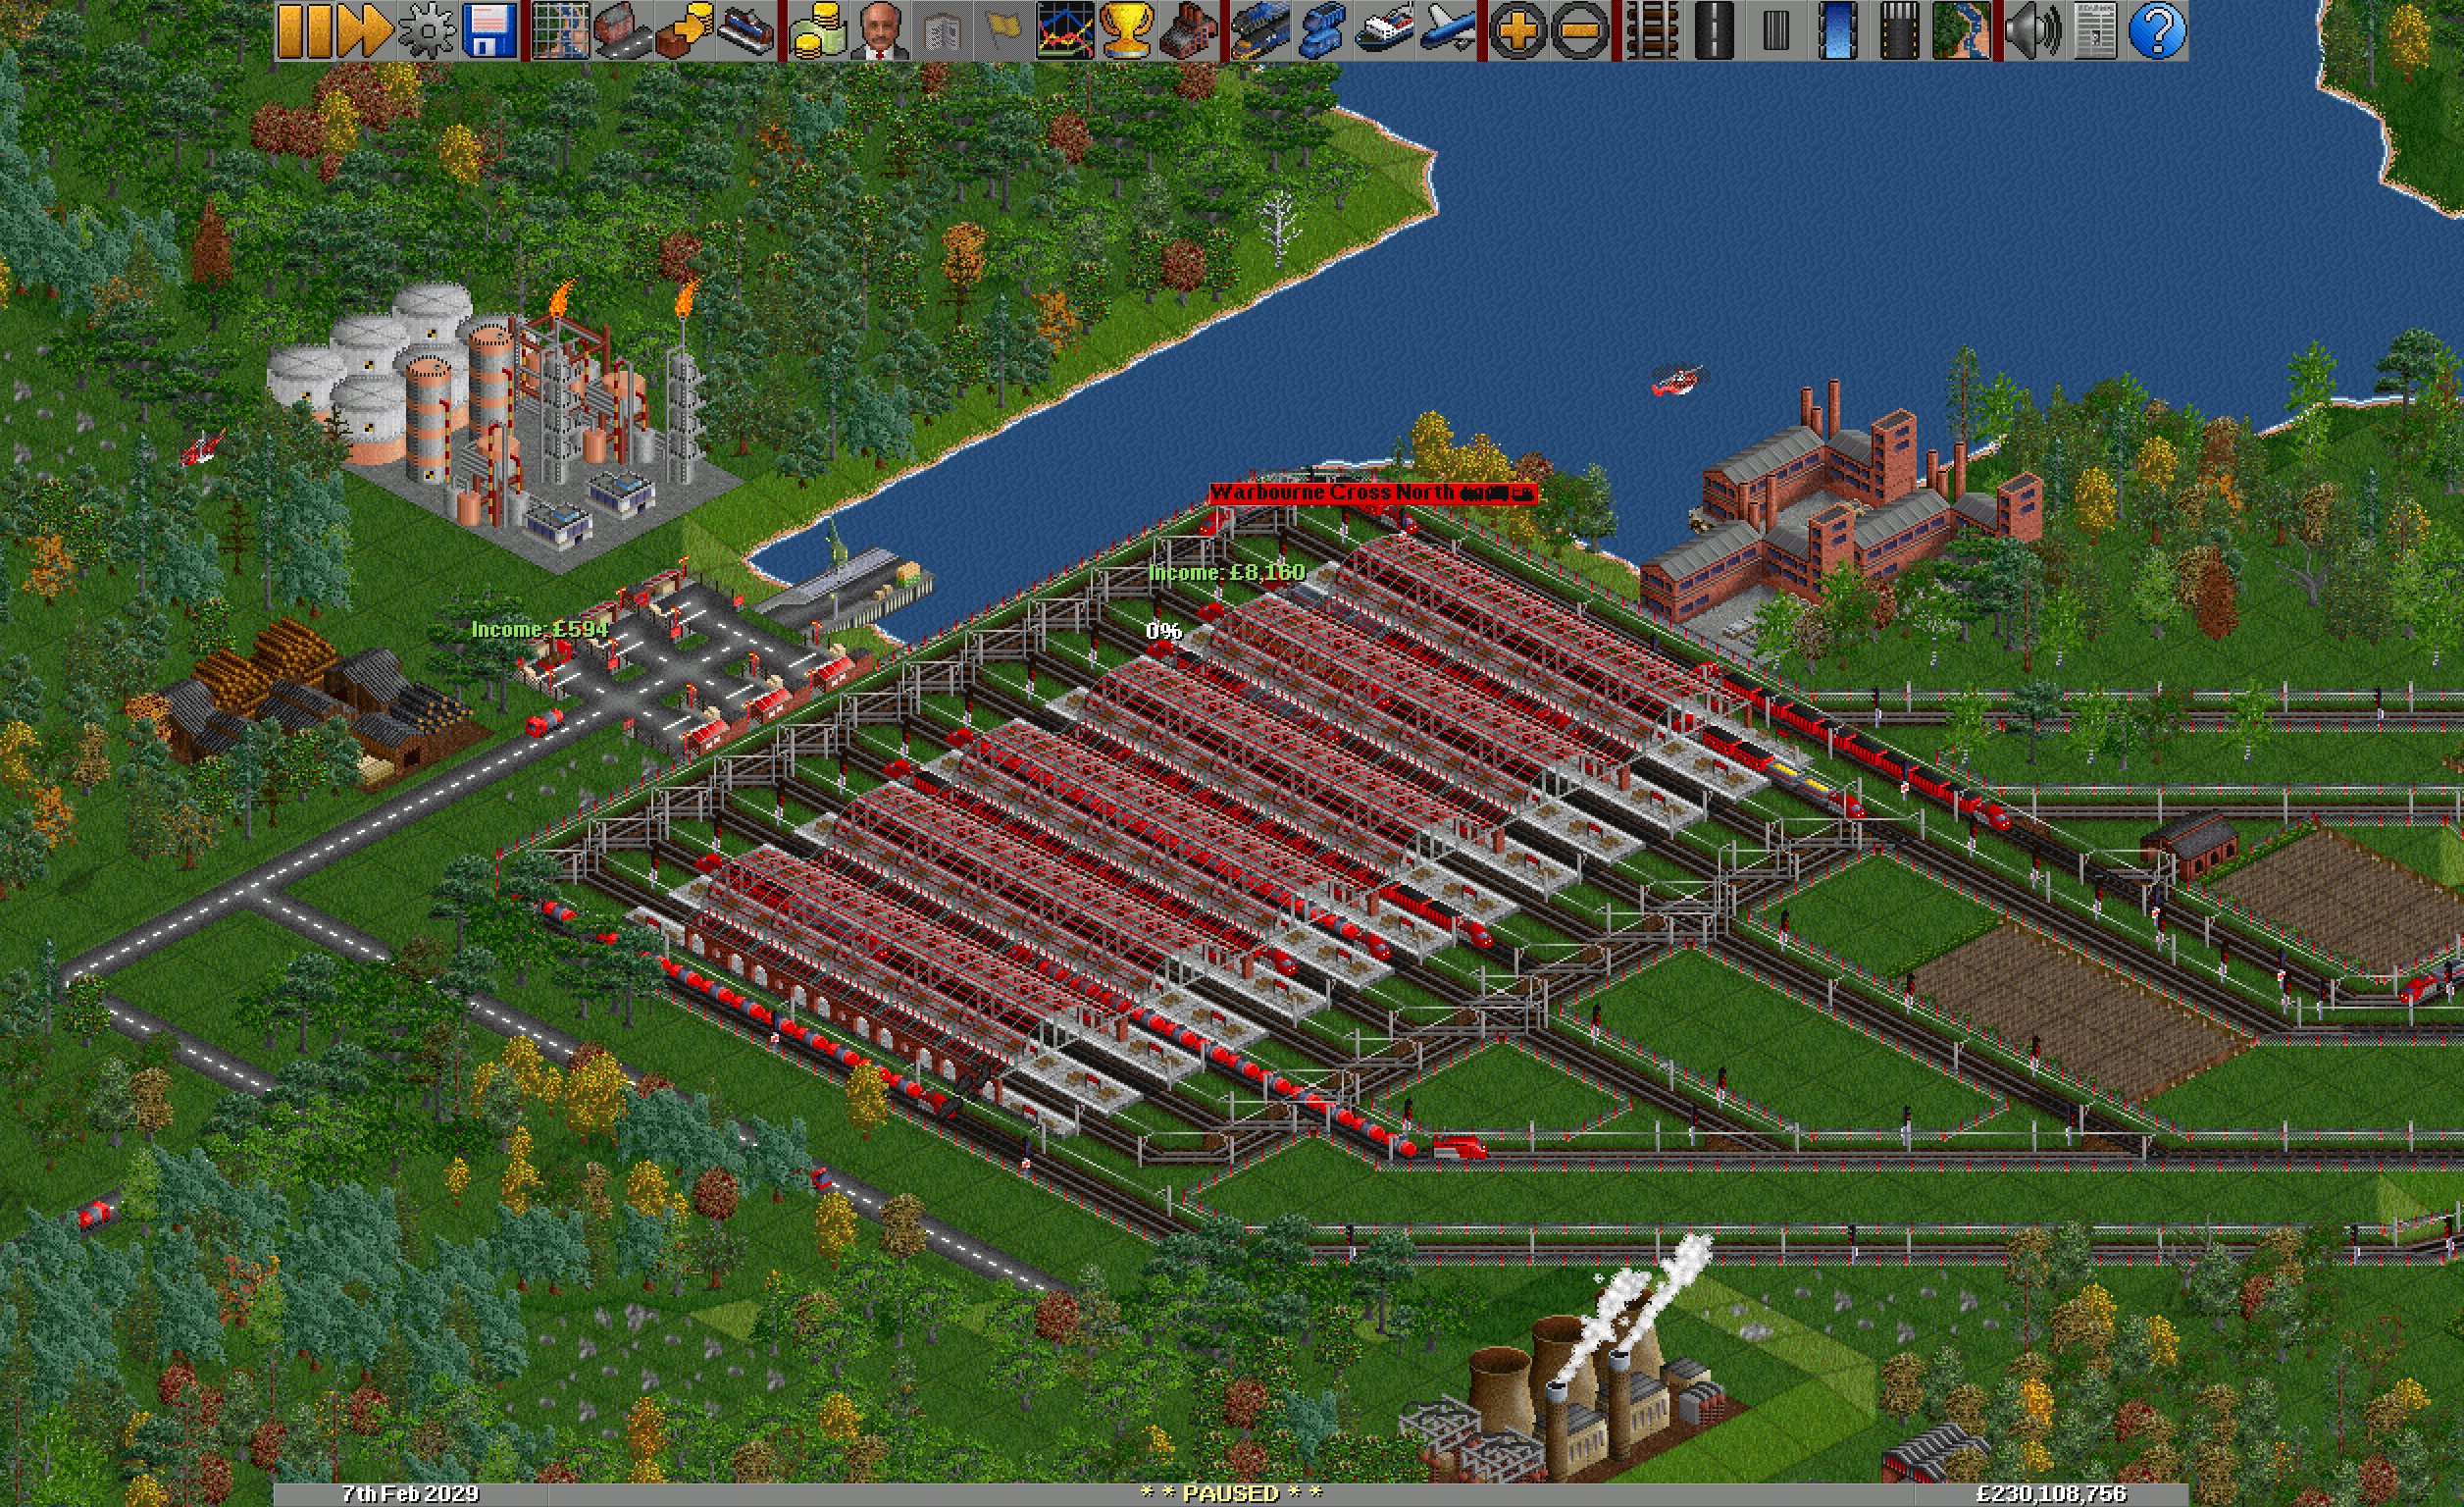
\includegraphics[width=\textwidth]{transport-tycoon-screenshot.png}
\caption{Screenshot of an OpenTTD game showing part of a transport network with multiple industries and mechanisms of transport. One of the trains has broken down, which not only prevents its cargo from reaching its destination, but it also prevents other trains from progressing along that track; OpenTTD has built-in ways of penalising non-resilience.}
\label{fig:network}
\end{figure}

OpenTTD is an open source business simulation game based on the 1990s game Transport Tycoon Deluxe. The aim of the game is to create a business that makes money from the transport of passengers and goods from one place to another, by constructing and using a network of road vehicles, trains, planes, or ships - also known as supply chains. An example of part of such a network can be seen in Figure \ref{fig:network}.

OpenTTD allows the implementation of so-called AIs, custom computer-based players that create their own supply chains to compete with human players. Over 50 such AIs have been created \cite{openttdAIs}. However, since OpenTTD is primarily a computer game rather than a tool for research, it is lacking in components for running reproducible experiments with such AIs and extracting data from them \cite{openttdNoHeadless}. The first aim of this project is to extend OpenTTD to allow such reproducible experiments.

The second aim of this project is to use OpenTTD and any extensions to construct an AI that allows the investigation of the links between resilience of such supply chains and other properties of the networks. And specifically, to help answer the question of when is it appropriate to build resilience into such networks. While the focus of this project is OpenTTD, results could be compared with investigations of real-world supply chains, and so adds to the body of research of such supply chains, and so could be used to inform government and corporate policies.

\subsection{Problem Statement}

The first problem is the problem than OpenTTD is not suitable to run reproducible experiments. While OpenTTD does have a dedicated server mode for multiplayer games, it is throttled to a speed for human players to interact with - it does no run at full speed. In addition, while OpenTTD does have the ability to autosave games, these are of a custom binary format and it is non trivial to extract metrics or topological details of the supply chains created.

The second problem is to answer the question \emph{When is it worth building in resilience into supply chains?} This is a broad question - it will not be able to be answered conclusively in the time available. However, it should be able to be answered in some limited extent, for example by focusing on highly simplified worlds, a single transport mechanism, simple supply chains of goods, or considering resilience only with respect to very limited events. Exactly what limitations will be applied will be chosen during the project.

\subsection{Research Hypothesis and Objectives}

Ideally, to make OpenTTD useful for reproducible research, any changes will be merged into its public repository \cite{openttdRepo}. These changes will make it straightforward, so in a very low number of commands or configuration changes, to run experiments over a range of scenarios or AIs. While OpenTTD is a game, players can play alone - and the AI playing alone affords reproducible experiments. OpenTDD has some of the configuration required, for example its \verb+-t+ command line argument can set a start year and \verb+-G+ can set a seed for the random number generator. However, it does not seem possible to set an end year after which OpenTTD will exit. It also had a  \verb+-D+ dedicated mode which runs the game without a graphical interface, but it's extremely throttled for human players to interact with which makes it unfeasible to use for more than a handful of experiments. Its \verb+-q+ argument can extract information from saved games to a text format, but the output is trivial. The objective of the first phase of the project will be to add suitable command line arguments to overcome these problems.

The second phase of the project, determining when its worth to build in resilience into networks, is more complex and open-ended. As an example, in OpenTTD you often have to choose between sending raw materials to a factory already in use with infrastructure already in place, or sending to another factory. The latter is more expensive, but offers protections against factories closing down. In this case the objective would be to answer the question on when it is worth that investment.

\subsection{Timeliness and Novelty}

While being based on a 1990s computer game, OpenTTD is actively developed and developed. For example, four releases have been made so far in 2023 \cite{openttdReleases}. And the study of supply chain resilience is an active area of research, especially following the coronavirus (COVID-19) pandemic that started in 2020 and the 2021 Suez Canal obstruction by the container ship Ever Given. A systematic literature survey on research into supply chains and COVID-19 \cite{moosavi_supply_2022} showed that ``resilience" was the top related keyword. However, the survey did not attempt to track changes over time. The results of a brief and informal analysis of published research indexed by Web of Science supply chain resilience is shown in Figure \ref{fig:supplychainresiliance} showing how supply chain research, and especially supply chain research mentioning the COVID-19 pandemic, is not just active, but an increasing area of research.

\begin{figure}[h]
\centering
\begin{gnuplot}[terminal=cairolatex,terminaloptions={size 6,3}]
set tics font ",5"
set ylabel 'Number of publications'
set xlabel 'Year'
set style data histograms
set style histogram rowstacked
set style fill pattern border -1
set xtics nomirror
set ytics 100
set key invert
set key left top
set grid ytics
set xtics font ", 5"
set ytics font ", 5"
plot 'supply-chain-resiliance-research.dat' \
    using 2 t "  Without COVID-19", \
    '' using 3:xticlabels(1) t "With COVID-19" lc rgb '#999999'
\end{gnuplot}
\caption{The number of publications indexed by Web of Science matching the topic ``supply chain resilience" between 2014 and 2022, showing the split between publications with the topic COVID-19, and publications without. Data retrieved April 2023.}
\label{fig:supplychainresiliance}
\end{figure}

In terms of novelty, the first phase of the project solves the reported \cite{openttdNoHeadless} deficiency in OpenTTD - repeatedly running experiments with a parameterised AI is a manual process. In the second phase, OpenTTD does not appear to have been used in the study of resilient supply chains - as of April 2023 no publications have been found indexed by Web of Science or Google Scholar linking OpenTTD with supply chain resilience.

\subsection{Significance}

The output of the first phase of the project, the headless mode of OpenTTD, is by itself valuable. Problems in existing research using OpenTTD include inconsistent time experiments are run for as in \cite{rios_trains_2009}, very few repetitions per case, such a 1 repetition per case in \cite{wisniewski_artificial}, and experiments using customised-but-unpublished versions of OpenTTD for research purposes in \cite{shen_rtsenv_2011, konijnendijk2015mcts}. The first phase will allow research to be easily done using OpenTTD in an automated and reproducible way that addresses all of these problems. 

The direct answer to the research question of the second phase is significant only in the  niche world of OpenTTD - its players and AI designers. However, the consequences of real-world supply chain disruptions can be serious: addressing this has been described as an ``urgent need" \cite{moosavi_supply_2022}. Thus, any details that could be applicable to real-world supply chains could be significant.


\subsection{Feasibility}

The fact that OpenTTD is open source allow changes to be made, and the 50 existing AIs suggest it's possible to make OpenTTD AIs using a variety of algorithms. I'm an experienced software engineer knowing several programming languages with experience of working in unknown codebases. Thus it is feasible for me to make changes to the source code, and to write an AI in the available time. OpenTTD is lightweight, and its AIs have limited computation available as discussed later, therefore resources are unlikely to require more than a standard laptop.

\subsection{Beneficiaries}

The first phase of the project should benefit researchers using OpenTTD for experiments, such as in \cite{rios_trains_2009, wisniewski_artificial, shen_rtsenv_2011}. Code will be published so it is openly available, with clear instructions on how to use it in order to reproduce results. The ideal output of the first phase is to allow researchers to reproduce any results in a single step, with any code changes merged into OpenTTD, so it will be ideally maintained for the lifetime of OpenTTD and easily discoverable by other researchers.

The second phase of the project, the beneficiaries would be players and writers of OpenTTD AIs, researchers into supply chains, and potentially, anyone that can be affected by issues in supply chains.

It is expected that during the use of OpenTTD for research, improvements will be made to its headless mode from the first phase as deficiencies are found. Even if the output of the second phase isn't directly useful, it should improve the usefulness of the first.

\section{Background and Related Work}

OpenTTD has a challenging computational environment:

\begin{enumerate}

\item OpenTTD is based on an isometric two dimensional grid, the default size of which is 512 $\times$ 512 = 262144 tiles. Each tile has approximately 100 individual actions. Plus, there are actions that take multiple map tiles, for example building a station that can cover multiple tiles as can be seen in Figure \ref{fig:network}. There are also actions that take place not directly on a tile, for example telling a vehicle to go to a particular station.

\item Even if it were theoretically computationally feasible to consider all possible actions, OpenTTD limits the number of computations an AI can take in any given amount of time.

\item The field of play is dynamic even if the AI chooses to take no action - calculated insights cannot be perfectly applied to the future because the map may have changed. This includes during construction of network components.

\item There are multiple scales involved - a higher level scale of deciding which goods to delivery where, but also a lower level as to where to place stations.

\end{enumerate}

Existing OpenTTD AIs attempt to overcome these issues in various ways. Very briefly, PathZilla \cite{pathzilla} uses Delaunay Triangulation combined with randomly choosing between towns and industries. The trAIns \cite{rios_trains_2009}  AI uses a modified version of the A* algorithm to plan routes between destinations. The AI in \cite{bijlsma2014evolving} uses a genetic algorithm approach to construct/choose rules to make its decisions. Any of these methods may be used to validate the first phase, or, if suitably modified, to generate results in the second.

While no publications have been found linking OpenTTD with supply chain resilience, supply chain resilience itself is well studied field. However, as of 2020 there does not appear to be an accepted definition of supply chain resilience, and studies on measuring it are ``scarce" \cite{doi:10.1080/00207543.2020.1785034}. A reasonable working definition is taken from \cite{kiers_which_2022}: ``Resilience is the ability of a system to detect, adapt, and react to disturbances to restore its original structure and functions" - a non-trivial concept to measure. Choosing appropriate metrics will be done during the second phase of the project.

\section{Programme and Methodology}

This project will be done primarily in 2 phases that I'm calling Reproducibility and Resilience. In addition to these, there will be a short initial Preparation phase.

\begin{enumerate}
\addtocounter{enumi}{-1}
    \item \textbf{Preparation}

    There will be an initial short preparation phase of this project is make sure I have a dissertation template - will be virtually empty at the beginning, and that I can compile OpenTTD and make basic changes, and create and run a trivial AI. If I'm unable to do any of these steps, this must be discovered very early on in order to change the later plan.
    
    \item \textbf{Reproducibility}

    The first main phase of the project focuses on making any required changes to OpenTTD in order to support reproducible research. This itself has two parts - a basic headless mode, and the construction of a naive AI developed using the headless mode. The purpose of the second part is to refine the headless mode in terms of usage and output, and to make sure that constructing an AI with certain properties is feasible in the time available.
    
    \item \textbf{Resilience}

    The second phase is to use the results of the previous phases to construct a parameterisable AI that can be used to investigate the relationship between properties of the networks it creates, and resilience of those networks.

    The exact form of this AI will depend on discoveries during the previous phases. For example, rail networks are particularly interesting due to break downs blocking networks as in Figure \ref{fig:network}, but are  difficult to construct due to signalling and de-facto one-way tracks.
    
\end{enumerate}

In terms of methodology, this project will be undertaken in a highly iterative way - tight cycles of development and evaluation. This is suitable since this is an ambitious project with a number of unknowns, mostly around how long activities will take. The cycles will include maintaining a ready to submit dissertation, as detailed in the next section.

\subsection{Risk Assessment}
\label{riskassessment}

For the first phase to give maximum value, any changes to OpenTTD would be merged into its codebase. However, there is no guarantee of this. Although OpenTTD is actively maintained, PRs remain open from 2019 \cite{openTTDPRs}, and its maintainers are under no obligation to merge them or any PRs submitted as part of this project. However, there are mitigations to this.

\begin{itemize}
    \item I'll submit changes as early as possible in the project.
    \item I'll submit changes that are as small as possible, and so more likely to be merged.
    \item I'll use what I submit as to make sure any changes are fit for purpose.
    \item I'll maintain my own fork while PRs are considered.
\end{itemize}

Overall, the biggest risk is running out of time without any useful output - software projects are overdue 60\% of the time \cite{chaos2015}. From my own experience as a software engineer, projects where the engineer is not familiar with the domain have the highest risk of this. This is such a project - I am not familiar with the OpenTTD codebase, and to date have not written an OpenTTD AI.

To mitigate this risk, I leverage the fact that while the submission deadline is fixed, what is submitted by that deadline is not, allowing me to take a multi-scale agile/iterative approach to the project and adjust its aim as it progresses if necessary. Specifically:

\begin{itemize}
    \item Each phase/iteration is a de-facto feasibility study for the next phase.
    \item Each phase/iteration will result in value in terms of novelty, timeliness, and significance.
    \item Each phase/iteration will result in a reasonably complete project at all times.
\end{itemize}

To reduce the need to trade-off ambition against leaving time to write up, the iterations include the deliverable dissertation itself. The dissertation will be started at the beginning of the project and maintained as the project progresses. This is a Continuous Delivery approach, and is often used when delivering web applications, for example \cite{chen_continuous_2015}. However, this approach has also been successfully used to include the delivery of the written component of doctoral dissertations \cite{alipui_agile_nodate}, so can be applied here. This approach also allows for doing less - if the project is enough for a good dissertation at any point, I can stop - this would be consistent with some of the results of \cite{alipui_agile_nodate} where some doctoral dissertations are submitted in a relatively short amount of time.

Figure \ref{fig:gantt} shows a Gantt chart of this process, and a summary of these risks are in Table \ref{fig:risks}.

\begin{table}[htbp]
    \begin{center}
        \begin{tabular}{|l|l|l|l|}
        \hline
        \textbf{Phases} & \textbf{Risk} & \textbf{Mitigations} & \textbf{Residual} \\
        \hline
        0, 1, 2 & Too time-consuming        & Earlier phase is feasibility study & Low \\
                &                           & Can expand on previous phases      & \\
                &                           & Re-plan                            & \\
        1       & Merges upstream take time & Initiate early                     & Low \\
                &                           & Make small, frequent changes       & \\
                &                           & Use what's submitted               & \\
                &                           & Maintain fork                      & \\
        2       & Non-reproducible results  & Create and use headless mode       & Low \\
                &                           & Maintain clear instructions        & \\
        \hline
        \end{tabular} 
    \end{center}
    \caption[Risks and mitigations]{Risks and mitigations}
    \label{fig:risks}
\end{table}

\subsection{Ethics}

All data will be generated during the project by simulations - there will be no data collected from individuals.

There are actions in OpenTTD that could be unethical if applied to the real world. For example, it is possible that an AI destroys buildings while making the network. The headless mode can be extended to allow reporting on such actions.

\subsection{Responsible Research}

The first phase of the project provides value, but it also exists to ensure that the second phase of the project produces results that are reproducible. As can be seen by the Gantt chart in Figure \ref{fig:gantt}, almost half of the project time will be dedicated to this. This is to limit the risk of the second phase becoming part of the so-called reproducibility crisis \cite{baker_1500_2016}.

\section{Evaluation}

The first phase of the project, making it easier for OpenTTD will be mostly qualitatively evaluated. Initially by myself, but ideally by OpenTTD maintainers who will decide whether to merge in any changes. There will also be an objective component - the number of manual steps required to be taken in order to reproduce research conducted with OpenTTD should be able to be counted before and after any changes.

The second phase of the project will use data extracted from OpenTTD, made possible from the first phase. For example tracking profit and topological properties of the networks.

\section{Expected Outcomes}

The outcome of the first phase of the project is that is will be easier to run reproducible experiments in OpenTTD. The second phase will use this output, refine it, and use it to help determine when it's worth building in resiliance of supply chains in OpenTTD.

\section{Research Plan, Milestones and Deliverables}

The discussed plan of work can be seen summarised in Figure \ref{fig:gantt}, with the milestones in Table \ref{table:milestones}, and deliverables in Table \ref{table:deliverables}. The project has approximately 16 months available, on a part time basis. Timelines are constructed based on my experience as a software engineer.

\begin{figure}[htbp]
\begin{ganttchart}[
    vgrid,inline,
    x unit=1cm,
    time slot format=isodate-yearmonth,
    time slot unit=month,
    title height=1,
    group peaks height=0,
    group left shift=0,
    group right shift=0,
    group top shift=.7,
    bar height=.6
   ]{2023-05}{2024-08}
    \gantttitlecalendar{year, month=shortname} \\
    \ganttbar[name=dissertation, bar label font=\footnotesize]{Dissertation}{2023-05}{2024-08} \\
    \ganttgroup{0 - Prep.}{2023-05}{2023-06} \\
    \ganttbar[name=compile, bar label font=\footnotesize]{Compilation}{2023-05}{2023-06} \\
    \ganttgroup{1 - Reproducibility}{2023-07}{2023-12} \\
    \ganttgroup[group height=.1]{Headless mode}{2023-07}{2023-09} \\
    \ganttbar[name=i1]{1}{2023-07}{2023-07} \ganttlink[link mid=.166666]{compile}{i1} \\
    \ganttbar[name=i2]{2}{2023-08}{2023-08} \ganttlink{i1}{i2} \\
    \ganttbar[name=i3]{3}{2023-09}{2023-09} \ganttlink{i2}{i3}  \\
    \ganttgroup[group height=.1]{Naive AI}{2023-10}{2023-12} \\
    \ganttbar[name=i4]{4}{2023-10}{2023-10} \ganttlink[link mid=.25]{i3}{i4} \\
    \ganttbar[name=i5]{5}{2023-11}{2023-11} \ganttlink{i4}{i5}   \\
    \ganttbar[name=i6]{6}{2023-12}{2023-12} \ganttlink{i5}{i6}   \\  
    \ganttgroup{2 - Resilience}{2024-01}{2024-08} \\
    \ganttgroup[group height=.1]{Parameterisable AI}{2024-01}{2024-08} \\
    \ganttbar[name=i7]{7}{2024-01}{2024-01} \ganttlink[link mid=.166666]{i6}{i7}  \\
    \ganttbar[name=i8]{8}{2024-02}{2024-02} \ganttlink{i7}{i8}  \\
    \ganttbar[name=i9]{9}{2024-03}{2024-03} \ganttlink{i8}{i9}  \\
    \ganttbar[name=i10]{10}{2024-04}{2024-04} \ganttlink{i9}{i10}  \\
    \ganttbar[name=i11]{11}{2024-05}{2024-05} \ganttlink{i10}{i11}  \\
    \ganttbar[name=i12]{12}{2024-06}{2024-06} \ganttlink{i11}{i12}  \\
    \ganttbar[name=i13]{13}{2024-07}{2024-07} \ganttlink{i12}{i13}  \\
    \ganttbar[name=i14]{14}{2024-08}{2024-08} \ganttlink{i13}{i14}
\end{ganttchart}
\caption[Project Gantt chart]{Gantt Chart of the activities defined for this project. This project will be undertaken on a part time basis and in a highly iterative way with at least 14 iterations. Each iteration will result in a complete project, but of limited scope, to be decided during each iteration.}
\label{fig:gantt}
\end{figure}

\begin{table}[htbp]
    \begin{center}
        \begin{tabular}{|S[table-format=2.0]|l|}
        \hline
    \textbf{Month} & \textbf{Milestone} \\
        \hline
        2 & Basic dissertation extended with the project \\
        2 & Can compile and make changes to OpenTTD \\
        5 & Headless mode created \\
        8 & Naive AI created along with refinements to headless mode \\
        16 & Complex AI created and used to investigate resilience \\
        \hline
        \end{tabular} 
    \end{center}
    \caption[Project milestones]{Project milestones}
    \label{table:milestones}
\end{table}
\begin{table}[htbp]
    \vspace{0.5cm}
    \begin{center}
        \begin{tabular}{|S[table-format=2.0]|l|}
        \hline
        \textbf{Month} & \textbf{Deliverable} \\
        \hline
        2 & Initial Dissertation \\
        5 & Initial headless mode \\
        8 & Naive AI as example of using headless mode \\
        16 & Parameterisable AI to investigate resilience \\
        16 & Final dissertation \\
        \hline
        \end{tabular} 
    \end{center}
    \caption[Project deliverables]{Project deliverables}
    \label{table:deliverables}
\end{table}

\pagebreak
%                Now build the reference list
\bibliographystyle{unsrt}   % The reference style
%                This is plain and unsorted, so in the order
%                they appear in the document.

{\small
\bibliography{main}       % bib file(s).
}
\end{document}

